% ------------------------------------------------------------------------ %
% !TEX encoding = UTF-8 Unicode
% !TEX TS-program = pdflatex
% !TEX root = ../Tesi.tex
% !TEX spellcheck = it-IT
% ------------------------------------------------------------------------ %
%
% ------------------------------------------------------------------------ %
% 	NOME CAPITOLO
% ------------------------------------------------------------------------ %
%
\chapter{Ethereum}
%
\label{cap:ethereum}
%
% ------------------------------------------------------------------------ %
%
\section{Introduzione e Smart Contracts}
%
Gli Smart Contract sono stati oggetto di sperimentazione già negli anni ’90 quando le tecnologie hanno permesso di attuare forme di sperimentazione di Smart Contract, ma l’idea di Contratto Intelligente risale in realtà alla metà degli Anni ’70. Il termine adottato all’epoca non era quello di Smart Contract, ma il concetto era sostanzialmente quello che ha portato ai contratti intelligenti. Infatti all’epoca l’esigenza atteneva alla necessità di gestire l'attivazione o disattivazione di una licenza software in funzione di alcune condizioni molto semplici. La licenza di determinati software venne di fatto gestita da una chiave digitale che permetteva il funzionamento del software se il cliente aveva pagato la licenza e ne cessava il funzionamento alla data di scadenza del contratto è stato il primo esempio di uno Smart Contract. \\
\emph{Ethereum}\autocite{eth} nasce invece nel 2013 per opera di Vitalik Buterin, uno sviluppatore di origini russe che ha unito la sua competenza di programmatore a quelle di ricercatore nell’ambito delle cryptocurrency. Lo scopo di Ethereum è quello di creare un protocollo alternativo per la costruzione di applicazioni decentralizzate in situazioni in cui sono essenziali: un tempo rapido di sviluppo, un alto gradi di sicurezza nelle applicazioni e la capacità di far interagire tra di loro in modo efficace applicazioni differenti. In definitiva, Ethereum è una blockchain con un linguaggio di programmazione costruito al suo interno, Turing completo, che permette a chiunque voglia di scrivere Smart Contracts e applicazioni decentralizzate (o DAPP) nelle quali è possibile stabilire:
\begin{itemize}
	\item le proprie regole di proprietà;
	\item i formati delle transazioni;
	\item le funzioni di transizione di stato.
\end{itemize}%
L’uso delle risorse computazionali di Ethereum è remunerato con una speciale “moneta virtuale” denominata \emph{Ether} che rappresenta essa stessa sia la potenza elaborativa necessaria per produrre i contratti sia la cryptovaluta che permette di “pagare” per la realizzazione dei contratti\footnote{in maniera simile a quanto avviene sulla blockchain di Bitcoin}. Ether è fondamentalmente un token che viene trattato come cryptocurrency exchange con il ticker symbol di ETC. \\
Una generica applicazione Ethereum decentralizzata può essere schematizzata ad alto livello nel seguente modo: 
\begin{center}%
	\begin{figure}[H]
		%
		\centering
		%
		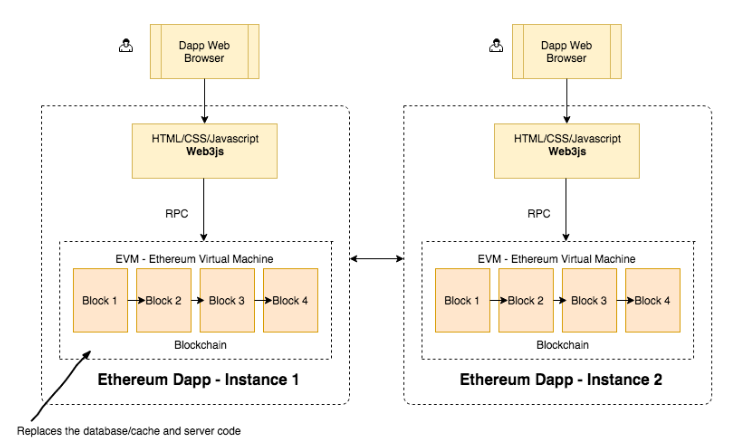
\includegraphics[width=.9\textwidth]{Ethereum/dapp}
		%
		\caption{Esempio di applicazione decentralizzata}
		%
		\label{fig:esempio di dapp}
		%
	\end{figure}
	%
\end{center}%
\section{Ethereum Accounts} 
%
In Ethereum, lo stato è costituito da oggetti chiamati \enquote*{accounts}. Ognuno di essi ha un indirizzo di 20 byte e le transizioni di stato sono trasferimenti diretti del valore e dell'informazione tra gli accounts. Un account Ethereum, è composto dai seguenti campi:
\begin{enumerate}
	\item il nonce: contatore utilizzato per assicurarsi che ogni transazione venga elaborata una sola volta;
	\item il bilancio ether: rappresenta il conto corrente dell'account;
	\item il contract code: il codice del contratto che può essere eseguito dai nodi della rete. Contiene funzioni che possono essere richiamato, perciò può essere paragonato ad un oggetto di un linguaggio object-oriented;
	\item lo storage dell'account.
\end{enumerate}%
In generale, esistono due tipi di accounts:
\begin{enumerate}
	\item \emph{accounts posseduti dall'esterno}: controllati da chiavi private. Questi non hanno codice ed è possono mandare messaggi esterni creando e firmando una transazione;
	\item \emph{accounts contratto}: controllati dal loro codice di contratto. Ogni volta che un account contratto riceve un messaggio (transazioni o messaggi) da altri contratti, il suo codice si attiva, permettendo a questo di leggere e scrivere verso uno storage interno e spedire altri messaggi oppure creare a sua volta contratti. \\ Sono controllati da chiavi private.
\end{enumerate}%
Quindi tutte le azioni sulla blockchain Ethereum sono innescate da transazioni inviate da account controllati esternamente. 
\begin{center}
	%
	\begin{figure}[H]
		%
		\centering
		%
		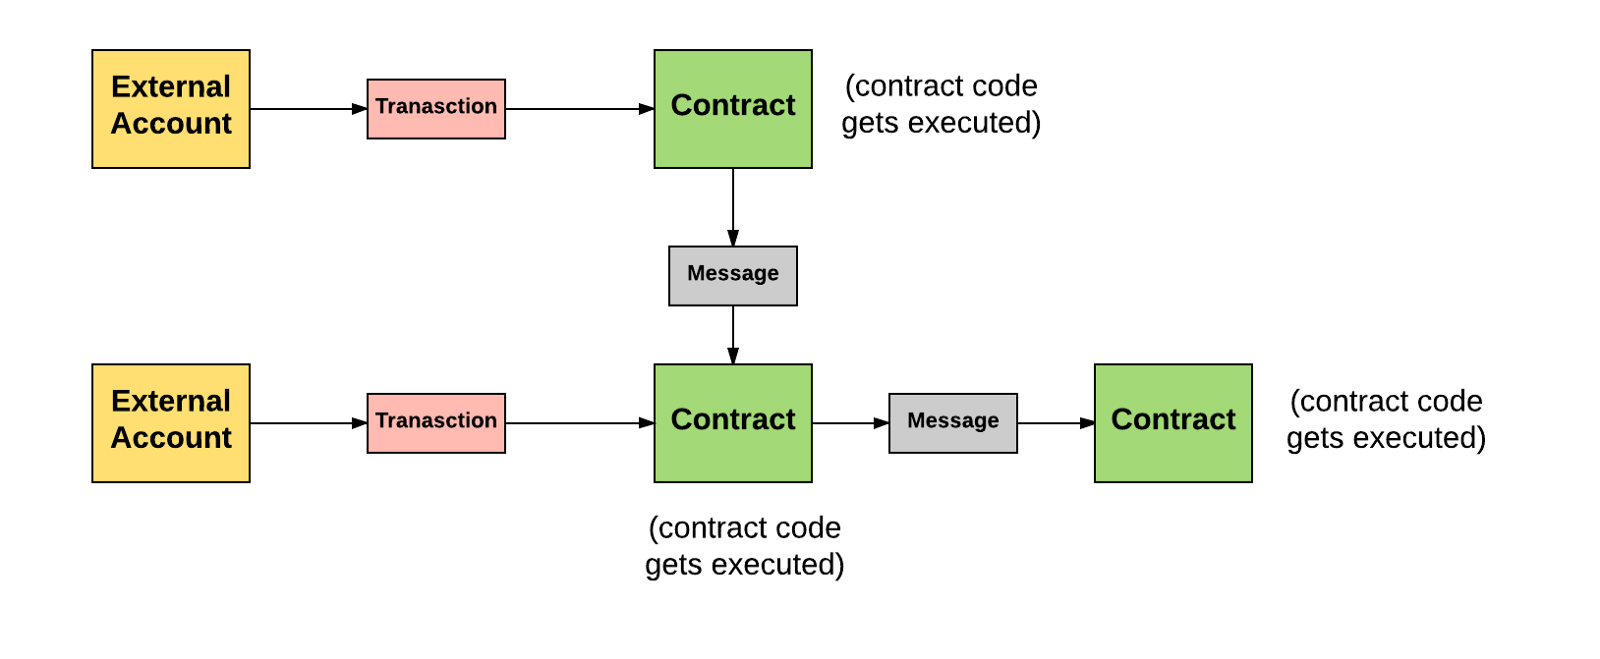
\includegraphics[width=.9\textwidth]{Ethereum/accounts}
		%
		\caption{Esempio di interazione tra accounts}
		%
		\label{fig:esempio di interazione tra accounts}
		%
	\end{figure}
	%
\end{center}
All'interno di Ethereum quindi gli account possono interagire tra di loro tramite messaggi oppure tramite transazioni.
%
\section{Messaggi e Transazioni}
%
\subsection{Transazioni}
%
Il termine \emph{transazione}, in Ethereum, viene utilizzato per riferirsi all'insieme di dati firmati che contengono un messaggio da inviare da un account posseduto dall'esterno. Le transazioni contengono:
\begin{enumerate}
	\item il destinatario del messaggio;
	\item una firma che identifica il mittente;
	\item l'ammontare di ether da trasferire al destinatario;
	\item un campo dati opzionale;
	\item un valore chiamato \emph{STARTGAS}: rappresenta il massimo numero di steps computazionali che l'esecuzione della transazione può impiegare;
	\item un valore chiamato \emph{GASPRICE}:  rappresenta la commissione che il mittente paga per lo step computazionale;
	\item v, r, s: usati per generare la firma che identifica il mittente della transazione.
\end{enumerate}
%
I campi (1.), (2.), (3.) sono campi standard previsti da qualsiasi criptovaluta. Il campo dati (4.) non ha una struttuda di default, potrebbe contenere un messaggio arbitrario oppure il codice per creare un contratto. Infatti la virtual machine di Ethereum ha un codice operativo con cui un contratto può accedere ai dati. Ad esempio, se un contratto sta funzionando come un servizio di gestione di ricette mediche basato su blockchain, potrebbe interpretare i campi che gli vengono passati come i campi della ricetta relativa in modo tale da poterli salvare correttamente nello storage. \\
I campi STARTGAS e GASPRICE sono essenziali per il modello di servizio anti-denial di Ethereum. Infatti al fine di prevenire loop infiniti, accidentali o malevoli che siano, o evitare spreco computazione di codice, ad ogni transazione è richiesto di impostare un limite per l'uso degli step computazionali di codice di esecuzione. L'unita fondamentale di computazione è il \emph{gas}. Solitamente uno step computazionale costa 1 gas ma potrebbe anche costa di più in quanto dipende dal livello di complessità computazionale delle operazioni o dalla quantità di dati che deve essere conservata come parte dello stato.\\
Infine, anche in Ethereum è presente una commissione (di gas) per ogni byte della transazione. Questa commissione ha uno scopo ben preciso, ovvero quello di obbligare un qualsiasi aggressore della rete a pagare proporzionalmente per ogni risorsa che essi vogliano consumare andando quindi ad includere la computazione, la larghezza di banda e lo storage.
%
\subsection{Messaggi}
%
I contratti hanno l'abilità di inviare "messaggi" ad altri contratti. I messaggi sono oggetti virtuali che non vengono mai serializzati ed esistono solo nell'ambiente di esecuzione di Ethereum (questi messaggi interni non sono quindi mai pubblicati sulla blockchain). Un messaggio è composto dai seguenti campi:
\begin{enumerate}
	\item il mittente del messaggio (implicito);
	\item il destinatario del messaggio;
	\item l'ammontare di ether da inviare attraverso il messaggio;
	\item un campo dati;
	\item un valore STARTGAS.
\end{enumerate}%
Un messaggio quindi è simile ad una transazione, eccetto che esso viene prodotto da un contratto e non da un attore esterno. Un messaggio viene prodotto quando un contratto che sta eseguendo il codice effetta una \emph{call}, che produce ed esegue appunto un messaggio. Come succede in una transazione, un messaggio comporta che l'account del destinatario esegua il proprio codice. In definitiva i contratti possono avere relazioni con altri contratti così come avviene con degli attori esterni e questo permette di avere un alto grado di libertà nella costruzione di applicazioni complesse. \\
In questo ambiente, la quantità di gas necessaria ad una transazione o ad un contratto, si applica alla totalità del gas consumato da quella transazione e da tutte le subesecuzioni. Ad esempio:
\begin{enumerate}
	\item un attore esterno A trasmette una transazione a B con 1000 gas;
	\item B consuma 600 gas prima di inviare il messaggio a C;
	\item C consuma internamente 300 gas prima di ritornare;
\end{enumerate}%
Dopo questi step B può spendere solo altri 100 gas prima di rimanere a corto di gas.
%
\section{Funzione Transazione di Stato}
%
Ethereum, quindi, si presenta come una macchina a stati basata sulle transazioni. Infatti quando una transazione viene eseguita all'interno della blockchain, la transizione verso uno stato finale rappresenta, in qualsiasi momento, lo stato attuale di Ethereum. Ad esempio nella seguente figura possiamo osservare la transizione da uno stato "State" ad uno stato "State'":
\begin{center}
	%
	\begin{figure}[h!]
		%
		\centering
		%
		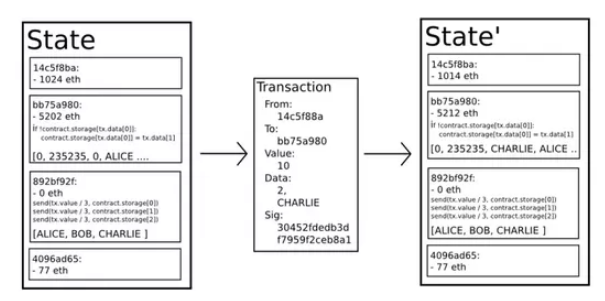
\includegraphics[width=.9\textwidth]{Ethereum/state}
		%
		\caption{Esempio di transizione di stato}
		%
		\label{fig:esempio di transazione di stato}
		%
	\end{figure}
	%
\end{center}
La funzione di transizione di stato di Ethereum può essere descritta, ad alto livello, nel seguente modo:
\begin{enumerate}
	\item controlla se la transazione è ben impostata (possiede il giusto numero di valori), se la firma è valida e il nonce corrisponde a quello dell'account del mittente. In caso contrario si verifica un abort;
	\item calcola la commissione di transazione come $STARTGAS*GASPRICE$ e determina l'indirizzo del mittente dalla firma. Sottrae poi la commissione dal bilancio dell'account del mittente e incremente il nonce del mittente. In caso in cui il bilancio da spendere sia insufficiente si verifica un abort;
	\item inizializza $GAS = STARGAS$ e toglie una certa quantità di gas per byte per pagare i byte della transazione;
	\item trasferisce il valore della transazione dall'account del mittente all'account del destinatario. Se l'account del destinatario non esiste ancora, lo crea. Se invece l'account destinatario è un contratto, esegue il codice del contratto per il completamento o fino all'esaurimento del gas;
	\item se il trasferimento del valore fallisce perchè il mittente non ha abbastanza soldi, il codice dell'esecuzione esaurisce il gas e ripristina tutti i cambiamenti di stato tranne che per il pagamento della commisione e aggiunge le stesse commissioni sul conto del minatore;
	\item se l'esecuzione termina correttamente, risarcisce al mittente le commissioni per il gas rimanente ed invia le commissioni pagate per il gas e consumante al miner.
\end{enumerate}%
\subsection{Esecuzione del Codice}
%
Il codice nei contratti Ethereum è scritto in un linguaggio di basso livello denominato \emph{codice virtual machine Ethereum} oppure \emph{codice EVM} che consiste in una serie di byte, dove ogni byte\footnote{in realtà il codice viene solo successivamente compilato in bytecode. Lo sviluppatore può servirsi di linguaggi di alto livello come Solidity o Serpent} rappresenta un'operazione eseguita all'interno dell'Ethereum Virtual Machine. \\ 
L'Ethereum Virtual Machine (EVM) è, quindi, l'ambiente di runtime per gli Smart Contract in Ethereum. L'ambiente risulta completamente sandboxato ed isolato il che significa che il codice in esecuzione al suo interno non ha accesso alla rete, al filesystem o ad altri processi. In generale, l'esecuzione del codice è un loop infinito che consiste nel realizzare ripetutamente l'operazione al contatore attuale del programma (che parte da 0) e incrementa il contatore di un'unità fino ad ottenere:
\begin{itemize}
	\item la fine del codice;
	\item un errore o STOP;
	\item viene rilevata l'istruzione RETURN.
\end{itemize}%
Le operazioni hanno accesso a tre tipi di spazio nel quale registrare i dati:
\begin{enumerate}
	\item Stack: un contenitore di tipo Last-In-First-Out (LIFO) nel quale i valori possono essere spinti;
	\item Memoria: un array di byte temporaneo (volatile) espandibile all'infinito;
	\item Storage: memoria non volatile mantenuta come parte dello stato e caratterizzata dall'essere di tipo chiave-valore.
\end{enumerate}%
La struttura dell'EVM è la seguente:
\begin{center}
	\begin{figure}[h!]
		%
		\centering
		%
		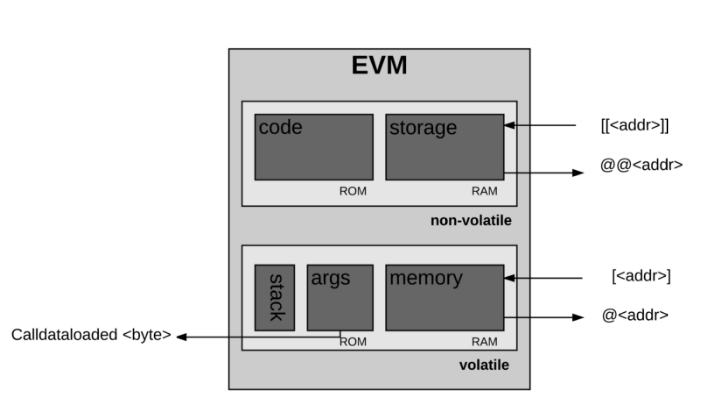
\includegraphics[width=.85\textwidth]{Ethereum/evm}
		%
		\caption{Schema dell'Ethereum Virtual Machine (EVM)}
		%
		\label{fig:schema dell'ethereum virtual machine}
		%
	\end{figure}
	%
\end{center}
Il modello di esecuzione formale del codice EVM risulta estremamente semplice. Infatti mentre la virtual machine di Ethereum funziona, tutto il suo stato computazionale può essere definito dall'insieme di dati (\emph{$stato_del_blocco$, transazione, messaggio, codice, memoria, stack, pc( i.e. program counter), gas}) dove $stato_del_blocco$ rappresenta lo stato globale che contiene tutti gli accounts e include i bilanci e lo storage. 
%
\section{Mining e Validazione}
%
Una volta validate, tutte le transazioni devono essere inserite in un blocco che deve essere anch'esso validato all'interno della rete. Un blocco (block header) in Ethereum si presenta nel seguente modo:
\begin{center}
	%
	\begin{figure}[h!]
		%
		\centering
		%
		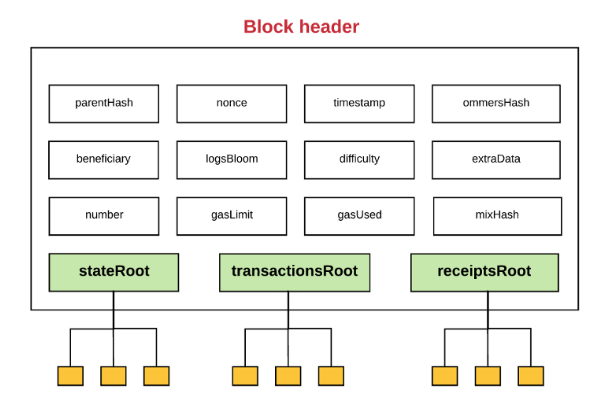
\includegraphics[width=.6\textwidth]{Ethereum/blockHeader}
		%
		\caption{Blocco in Ethereum}
		%
		\label{fig:blocco in Ethereum}
		%
	\end{figure}
	%
\end{center}
Per una descrizione dettagliata della struttura del block header si rimanda all'\autoref{cap:blockheader}. \\
L'algoritmo di validazione del blocco in Ethereum funziona nel seguente modo:
\begin{itemize}
	\item controlla se il precedente di riferimento essite ed è valido;
	\item controlla se la marca temporale del blocco è più grande di quella del blocco di riferimento precedente ed inferiore a 15 minuti nel futuro;
	\item controlla se il numero di blocco, la difficoltà del blocco, il transaction root, l'uncle root e il GASLIMIT sono validi;
	\item controlla se la proof-of-work sul blocco sia valida;
	\item sia $S[0]$ lo stato finale del blocco precedente;
	\item sia data la lista TX delle transazioni del blocco, con \emph{n} transazioni. Per tutti $i$ in $0..n-1$ sia $S[i+1]$ il risultato dell'applicazione della funzione transazione di stato sulla $TX[i]$ (ovvero ottengo il nuovo stato finale).\\ Viene restituito un errore in caso di superamento del GASLIMIT o in caso di errore dell'applicazione;
	\item sia lo stato finale $S[n]$ aggiungendo però la ricompensa per il blocco pagata al miner;
	\item l'algoritmo controlla che il root state del merkle tree sia uguale allo state root finale fornito nell'intestazione del blocco. Se i due valori corrispondono il blocco viene dichiarato valido. 
\end{itemize}%
Come in Bitcoin, anche in Ethereum la fase del mining passa attraverso la proof-of-work chiamata "Ethash" (conosciuta precedentemente come Dagger-Hashimoto)\cite{dh}. \\ L'algoritmo di valutazione, che a prima vista potrebbe sembrare inefficiente dato che registra l'intero stato di ogni blocco, risulta a livello di efficienza comparabile con quella di Bitcoin. Questo perchè lo stato viene registrato in una struttura ad albero e dopo ogni blocco solo una minima parte dell'albero necessita di essere cambiata. Quindi, in generale, tra due blocchi adiacenti la grande maggioranza dell'albero dovrà essere la stessa e quindi i dati possono essere registrati solo una volta e referenziati due volta tramite puntatori (ad es. gli hash degli alberi inferiori). Per raggiungere tutto questo Ethereum utilizza un tipo di albero conosciuto come \emph{Patricia Tree}\footnote{Permette ai nodi di essere non solo modificati con efficienza, ma anche inseriti e cancellati} , che consiste in una modifica ai Merkle Tree descritti in precedenza. Inoltre dato che tutta l'informazione sullo stato è una parte dell'ultimo blocco, non c'è bisogno di registrare tutta la storia della blockchain (ulteriore punto a favore rispetto alla blockchain di Bitcoin). 
%
